% !TeX root = ../msc_thesis_jayd.tex
\chapter{Introduction}

Our story begins, as most stories do, with a simple premise. 
Circa 1878, John William Strutt, Third Baron Rayleigh -- Lord Rayleigh, for short -- 
observed a peculiar phenomena in 
St Paul's Cathedral: a small whisper, uttered from one side of the circular
gallery, could be heard quite clearly by anyone seated along the outer edge of the gallery
and even travel back to the ears of the whisperer.
To explain his observation, Lord Rayleigh borrowed from geometrical optics
and modeled the sound waves as packets, or particles, of sound that undergo
specular reflection upon contact with the wall \cite[\S287]{RAY1878}. 
This picture, akin to the trajectories of billiard balls, allowed him to 
conclude that ``sonorous vibrations have a tendency to cling to a concave surface''.
This billiard analysis is later complemented by a complete wave analysis wherein 
he shows that the equation of aerial vibrations, essentially Helmholtz's equation, 
admit solutions of the form
  \begin{equation*}
   \psi_n(r,\theta,t)=J_n(kr)\cos(kat-n\theta)
  \end{equation*}
and that most of the amplitude, for a certain range of parameters (specifically, $n\gg kr$), 
is concentrated within an annulus near the boundary of the gallery \cite{RAY1910}, 
further proving his explanation.
He also noted that his derivation held for electrical waves if the walls
were perfectly conducting. He termed this phenomenon the whispering-gallery 
phenomenon and, today, we call this type of waves whispering-gallery waves
\index{whispering-gallery}.

Our journey thus begins on the wings of the whisper, forever gliding
along the concave surface of a perfectly smooth wall. However, no 
journey worth recounting happens without any bumps in the road.

\section{The Study of Passive Dielectric Microcavities}

For the better part of the 20\textsuperscript{th} century, the whispering-gallery 
phenomenon remained only a matter of curiosity \cite{WRI2012}. It was brought
back to light in the mid-1980s when it was realized that \textit{dielectric resonators}
\index{dielectric resonators}
had the potential to attain unparalleled electromagnetic energy storage
capabilities via the use of whispering-gallery modes (WGM) \cite{YAM1993}.
Research in this area increased exponentially when their application as 
extremely sensitive biosensors was theoretically explored 
and later experimentally achieved \cite{SER95,VOL2002,ARM2003,VOL2008}.

The whispering-gallery phenomenon in dielectric media can be explained
via the same basic physics as the whispering gallery of St Paul's Cathedral, 
but with a crucial difference: the mechanism by which the light (or sound) is confined.
Both the cathedral and the metallic sphere described by Lord Rayleigh as known as 
\textit{closed cavities}: the whisper does not leave the interior of the gallery,
as the electric field does not leave the confines of its metallic prison due to the perfect
reflections at the boundary. The walls of the cavity do not allow the waves to penetrate their depth. 
On the other hand, dielectric cavities retain light by way of \textit{total internal reflection}, which
implies the existence of an evanescent wave normal to the boundary, which in turn
allows the wave to leak, or couple, to the exterior of the cavity. This has multiple
experimental and theoretical consequences, which we will explore in this essay.

% We need layers to draw the block diagram
\pgfdeclarelayer{background}
\pgfdeclarelayer{foreground}
\pgfsetlayers{background,main,foreground}

\begin{figure}
  \centering
  \begin{subfigure}[b]{0.45\textwidth}
    \begin{center}
    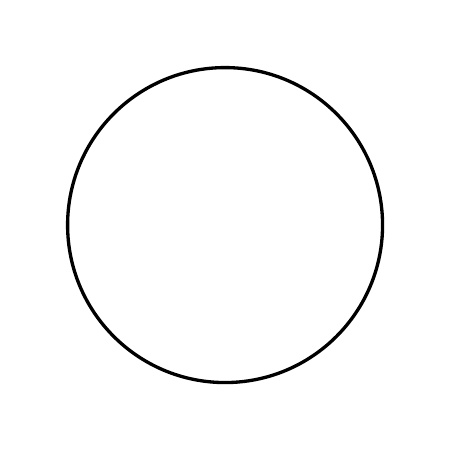
\begin{tikzpicture}
      \draw[very thick,fill=white] (0,0) circle (2);
      %\inscribedPolygon{2}{7}{0}
      \inscribedPolygon{2}{8}{25}
      %\inscribedPolygon{2}{6}{50}
      %\inscribedPolygon{2}{8}{75}
      %\inscribedPolygon{2}{9}{90}

      \begin{pgfonlayer}{background}
	\draw[white,inner color=white] (0,0) circle (2.5);
      \end{pgfonlayer}
    \end{tikzpicture}
    \end{center}
  \caption{Closed cavity with a WGM of quantum number $m=8$.}
  \end{subfigure}
  \begin{subfigure}[b]{0.45\textwidth}
    \begin{center}
    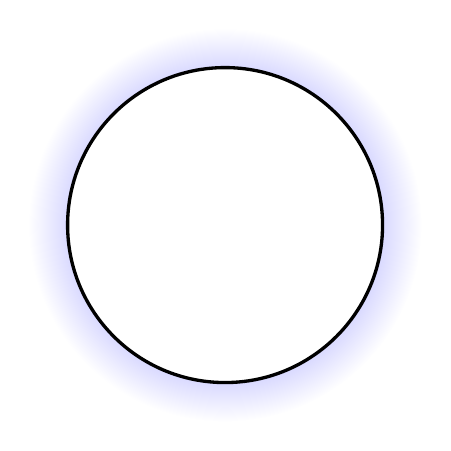
\begin{tikzpicture}
      \draw[very thick,fill=white] (0,0) circle (2);
      %\inscribedPolygon{2}{7}{0}
      %\inscribedPolygon{2}{8}{25}
      %\inscribedPolygon{2}{6}{50}
      %\inscribedPolygon{2}{8}{75}
      \inscribedPolygon{2}{9}{90}

      \begin{pgfonlayer}{background}
	\draw[white,inner color=blue!75] (0,0) circle (2.5);
      \end{pgfonlayer}
    \end{tikzpicture}
    \end{center}
  \caption{Open cavity with a WGM of quantum number $m=9$.}
  \end{subfigure}

\caption[Schematic representation of whispering-gallery modes]
	{Schematic representation of whispering-gallery modes in closed
	and open resonators. In closed resonators, WGMs have infinite lifetimes
	as they cannot interact with the external world. In open cavities, evanescent
	leakage (represented by the blue glow), implies interaction with the environment, which
	implies finite modal lifetime.}
\label{fig:intro.whisperingGalleryWaves}
\end{figure}

Mathematically, closed cavities usually obey Helmholtz's equation
  \begin{equation}
   \left[\nabla^2+k^2\right]\psi=0\qquad \psi(\bo{r}\in\mathcal{C})=0
  \end{equation}
where $\psi$ is the oscillation (pressure field, electric field, etc.)
and $\mathcal{C}$ is the boundary of the cavity. This partial differential
equation\index{partial differential equation} together with the \gls{dirichletBC} translates to an
eigenvalue problem: solutions only exist for a discrete set of eigenvalues 
$k_n$. These closed cavities have been a testbed for theoretical
and experimental endeavours in the last three decades, as can be
seen from the great amount of work done in the fields of quantum 
chaos and random matrix theory (RMT), for instance. Quantum chaos attempts
to classify the chaotic eigenstates of systems with non-separable Schrödinger
equations using the underlying (semi-)classical mechanics of the 
cavity \cite{BLU1990}. Research in this area helps to define the classical-quantum
transition. Level-spacing statistics of closed cavities also provides
a way to classify the eigenstates, depending on the statistical 
ensemble the cavity falls into. 

Closed cavities, are, however, an idealization of the much more
realistic open cavity. The discrete states of the former exist 
indefinitely inside the cavity; they have an infinite lifetime. 
They thus have infinite energy storage capabilities, but are impossible 
to generate. Open cavities, which also obey Helmholtz equation, but with the 
Sommerfeld radiation condition\index{Sommerfeld radiation condition} (a \gls{robinBC})
  \begin{equation}
   \lim_{r\rightarrow\infty}r^{\frac{d-1}{2}}\left(\frac{\partial}{\partial r}-ik\right)\psi=0
  \end{equation}
have a continuum of solutions. A countably infinite set of resonances\index{resonance}
can be defined for those cavities. These resonances have finite lifetimes.
The lifetimes are usually quantitatively described by the quality
factor, or $Q$-factor\index{$Q$-factor}, which is defined via the positions of the poles
on the complex $k$-plane 
	\begin{equation}
		Q = \frac{\Re{k_p}}{\left|2\Im{k_p}\right|}
	\end{equation}
and can be interpreted as the time it takes the light to escape the 
cavity. Experimentally, it is related to the finesse of the resonance. 
In an experimental scattering event, the transmission spectrum shows
a Lorentzian dip of width $\delta\lambda$. The $Q$-factor can thence
also be written
	\begin{equation}
		Q = \frac{\delta\lambda}{\lambda}.
	\end{equation}
An incoming field from infinity can interact with the modes of the
cavity and then escape the confines of the cavity. The \textit{tim-delay}\index{time-delay} introduced
by the interaction is linked to the lifetime of the modes of the cavity. 

This rather pictorial viewpoint can be made formal by the use of \textit{scattering theory}\index{scattering theory}, 
in which we suppose that a field, coming from infinity, suffers some changes due to its
interaction with the cavity and escapes to infinity once again. The object that we will consider
is the \gls{sMatrix}, which describes the relationship between the field after the interaction
and the field before the interaction, i.e. it describes the effect of the potential
on an incoming field. The scattering approach allows us to define the modes of 
open cavities, a problem that is perhaps more complicated that it seems \cite{DUT2000,DUT2001,TUR2005}.

Open dielectric cavities also allow a semi-classical approximation, mathematically
obtained by letting the wavelength $\lambda$ to be very small compared to 
the characteristic lengths involved in the system, or $k\rightarrow\infty$. 
The resulting open billiard can and has been used to engineer the cavities
to specific purposes \cite{KIM2013}. The fact
that the resulting system is Hamiltonian (but not necessarily Hermitian) 
has been used to study open quantum systems and non-Hermitian quantum 
mechanics experimentally \cite{BIT2010}. This stems from the similarities between the
Helmholtz and Schrödinger equations. Since the billiard system is Hamiltonian, 
one can set up a phase space with Birkhoff coordinates \cite{BIR1927}. 
Using the Husimi \cite{LEE1995} transform, this can be used to test
the phase-space formulation of quantum mechanics \cite{ZUR2003}.

Most applications of open dielectric cavities urge the use of very high $Q$
resonances. In WGM biosensors, the $Q$ value dictates the performance
of the sensor; in microlasers, it means a better field enhancement; in cavity
QED, higher $Q$ and lower mode volumes make it possible to study the quantum 
effects of light-matter interaction. It is possible to experimentally obtain
values of $Q\sim10^7-10^9$ using highly symmetrical cavity designs \cite{ARM2003,ARM2007,WAR2011}.
This symmetry implies that the far-field emission is also symmetric: it is
isotropic. For some applications, such as some designs of WGM biosensors, this may be
fine. However, for lasing applications, one would like to have, simultaneously, 
high-$Q$ and directionality in the far-field emission. The duality of those 
two concepts is one of the many facets of the study of \glspl{arc}, dielectric
cavities that are parametrically deformed versions of the circular cavity. 
This allows a certain degree of freedom in the design of microcavities and has
lead to interesting phenomena, such as exceptional points \cite{DET2009,RYU2009,HEI2012,BIT2014}, 
avoided crossings \cite{SON2013}, Goos-Hänchel shift \cite{UNT2008}, among others.

In this essay, we will use a second degree of freedom in the design
by allowing the refractive index distribution to be completely
arbitrary inside the cavity. This new degree of freedom can be realized
experimentally by the use of nematics \cite{PTA2013}. 
Moreover, we will see that the numerical
methods developed in this context could also be used to better model the lasing 
operation of active dielectric cavities.

\section{Onwards to Radiating Structures}
The expertise developed in the study of dielectric cavities is then
extended to lasing cavities and proposed for arbitrary
3D structures. We will touch upon the modelization of active
dielectric cavities with the use of \gls{salt}\index{SALT} which, as its name
hints, provides a steady-state model for the behaviour of the 
active medium. The particular set of approximations used 
allow to model the population dynamics of quantum $N$-level
systems as a static, but possibly spatially-varying and non-linear, 
modification of the refractive index of the passive cavity. 
In the linear case, basis expansions methods (such as the ones
we use) can be applied. We will a more stable numerical method
based on the Lippmann-Schwinger version of Helmholtz's equation.

We will also discuss the application of the method to arbitrary 
3D structures. We will attempt to model a type of antennae 
called \glspl{lcx}\index{leaky coax}. Their highly non-trivial geometry and the specifics
of their experimental realization will make our method rather hard 
to implement in that case. We will thus use all-numerical methods 
to extract the necessary information. Proper introduction to this project
will be given later.

\section{Content of this Essay}

In first chapter of this essay, we detail our work on open
dielectric cavities with arbitrary refractive index profiles. 
We generalize a scattering method by G.P.-A. \cite{GAP2013a} for 
complex refractive indices and TE polarization. We first describe
the analytical formalism and develop some of the scattering theory 
that is needed. We then discuss the development and numerical implementation
of the solution of Helmholtz's equation in inhomogeneous cavities. 
We then showcase the method by analyzing a circular microcavity with a 
Gaussian deformation of its refractive index. 

The second chapter discuss the extension to lasing structures and briefly
discusses the Lippmann-Schwinger method. We then model a family of \glspl{lcx}
with the \gls{fem}. Most of the work done aimed to conciliate the 
experimental and theoretical data sets, mainly by explaining the source
of the discrepancy. The effects of several physical parameters were thus explored. 

% In this master's thesis, we are concerned with making proper use of analytical
% and numerical methods and revealing the tension that exists between the two. 
% 
% In the first part, the analysis can be taken far enough as to warrant the
% development of a numerical method. In fact, we will generalize
% a known method to complex refractive indices and TE polarization. 
% 
% \todo[inline]%
% {%
%   Comparison of our  methods to quantum scattering.
%   Use of quantum scattering methods $\psi \sim e^{ikr}+e^{-ikr+\delta_\ell}$ 
%   to define the scattering matrix. Derivation of Q-matrix in quantum and 
%   electromagnetic cases (heuristic justification for $S^{-1}$ in complex case).
%   Quantum version of variable phase method (diagonal matrix case) as guide
%   to electromagnetic one. Boundary conditions?
% }%
% 
% \begin{itemize}
%  \item Whispering Gallery Modes
%   \begin{itemize}
%     \item Properties of WGMs
%     \item Applications to biosensing
%       \begin{itemize}
% 	\item Displacement of resonant $\lambda$
% 	\item Other mechanisms
%       \end{itemize}
%    \item Applications to microlasers
%       \begin{itemize}
% 	\item Directional Emission vs high-$Q$ operation
% 	\item Modeling of Asymmetric Resonant Cavities
%       \end{itemize}
%   \end{itemize}
%   \item ARCs
%     \begin{itemize}
%       \item Ray vs wave picture
%       \item Engineering of QB states
%       \item Laser operation and SALT
%     \end{itemize}
%   \item Antennae
%     \begin{itemize}
%       \item Scattering Methods for Radiating Structures
%       \item All-numerical methods and their (dis)advantages.
%     \end{itemize}
% \end{itemize}
